\begin{exercises} 

\item \label{Ez:1.1.1} A bungee jumper dives from a tower at time $t=0$.   Her height $h$ (measured in feet) at time $t$ (in seconds) is given by the graph in Figure~\ref{F:1.1.Ez1}.

\begin{figure}[h]
\begin{center}
 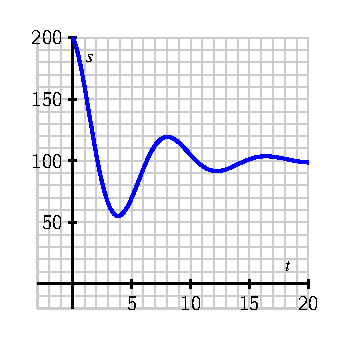
\includegraphics{figures/1_1_Ez1.eps}
 \caption{A bungee jumper's height function.} \label{F:1.1.Ez1}
\end{center}
\end{figure}

In this problem, you may base your answers on estimates from the graph or use the fact that the jumper's height function is given by $s(t) = 100\cos(0.75t) \cdot e^{-0.2t}+100$.
  \ba
	\item What is the change in vertical position of the bungee jumper between $t=0$ and $t=15$?
	\item Estimate the jumper's average velocity on each of the following time intervals:  $[0,15]$, $[0,2]$, $[1,6]$, and $[8,10]$.  Include units on your answers.
	\item On what time interval(s) do you think the bungee jumper achieves her greatest average velocity?  Why? 
	\item Estimate the jumper's instantaneous velocity at $t=5$.  Show your work and explain your reasoning, and include units on your answer.
	\item Among the average and instantaneous velocities you computed in earlier questions, which are positive and which are negative?  What does negative velocity indicate?
  \ea 

\begin{exerciseSolution}
\end{exerciseSolution}
\item A diver leaps from a 3 meter springboard.  His feet leave the board at time $t=0$, he reaches his maximum height of 4.5 m at $t = 1.1$ seconds, and enters the water at $t = 2.45$.  Once in the water, the diver coasts to the bottom of the pool (depth 3.5 m), touches bottom at $t=7$, rests for one second, and then pushes off the bottom.  From there he coasts to the surface, and takes his first breath at $t=13$.

\ba
  \item Let $s(t)$ denote the function that gives the height of the diver's feet (in meters) above the water at time $t$.  (Note that the ``height'' of the bottom of the pool is $-3.5$ meters.)  Sketch a carefully labeled graph of $s(t)$ on the provided axes in Figure~\ref{F:1.1.Ez2}.  Include scale and units on the vertical axis.  Be as detailed as possible.

\begin{figure}[h]
  \begin{center}
 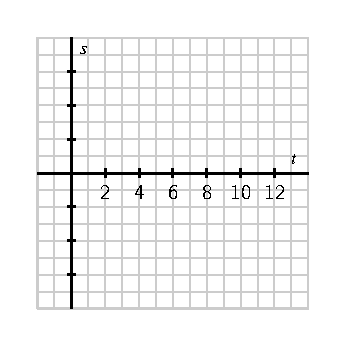
\includegraphics{figures/1_1_Ez2a.eps} \ \  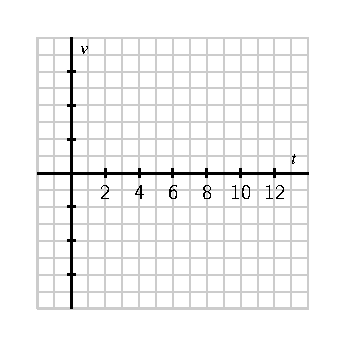
\includegraphics{figures/1_1_Ez2b.eps}
   \end{center}
   \caption{Axes for plotting $s(t)$ in part (a) and $v(t)$ in part (c) of the diver problem.} \label{F:1.1.Ez2}
\end{figure}

  \item Based on your graph in (a), what is the average velocity of the diver between $t = 2.45$ and $t=7$?  Is his average velocity the same on every time interval within $[2.45,7]$? 

  \item Let the function $v(t)$ represent the \emph{instantaneous vertical velocity} of the diver at time $t$ (i.e.~the speed at which the height function $s(t)$ is changing; note that velocity in the upward direction is positive, while the velocity of a falling object is negative).  Based on your understanding of the diver's behavior, as well as your graph of the position function, sketch a carefully labeled graph of $v(t)$ on the axes provided  in Figure~\ref{F:1.1.Ez2}.  Include scale and units on the vertical axis.  Write several sentences that explain how you constructed your graph, discussing when you expect $v(t)$ to be zero, positive, negative, relatively large, and relatively small.
  \item Is there a connection between the two graphs that you can describe?  What can you say about the velocity graph when the height function is increasing?  decreasing?  Make as many observations as you can.
\ea
\begin{exerciseSolution}
\end{exerciseSolution}

\item According to the U.S. census, the population of the city of Grand Rapids, MI, was 181,843 in 1980; 189,126 in 1990; and 197,800 in 2000.

\ba
	\item Between 1980 and 2000, by how many people did the population of Grand Rapids grow?
	\item In an average year between 1980 and 2000, by how many people did the population of Grand Rapids grow?
	\item Just like we can find the average velocity of a moving body by computing change in position over change in time, we can compute the average rate of change of any function $f$.  In particular, the \emph{average rate of change} of a function $f$ over an interval $[a,b]$ is the quotient
$$\frac{f(b)-f(a)}{b-a}.$$  
What does the quantity $\frac{f(b)-f(a)}{b-a}$ measure on the graph of $y = f(x)$ over the interval $[a,b]$?
	\item Let $P(t)$ represent the population of Grand Rapids at time $t$, where $t$ is measured in years from January 1, 1980.  What is the average rate of change of $P$ on the interval $t = 0$ to $t = 20$?  What are the units on this quantity?
	\item If we assume the population of Grand Rapids is growing at a rate of approximately 4\% per decade,  we can model the population function with the formula $$P(t) = 181843 (1.04)^{t/10}.$$  Use this formula to compute the average rate of change of the population on the intervals $[5,10]$, $[5,9]$, $[5,8]$, $[5,7]$, and $[5,6]$.
	\item How fast do you think the population of Grand Rapids was changing on January 1, 1985?  Said differently, at what rate do you think people were being added to the population of Grand Rapids as of January 1, 1985?  How many additional people should the city have expected in the following year?  Why?
\ea

\end{exercises}
\afterexercises
